\section{\ourmethod}
\begin{figure}[t]
    \centering
    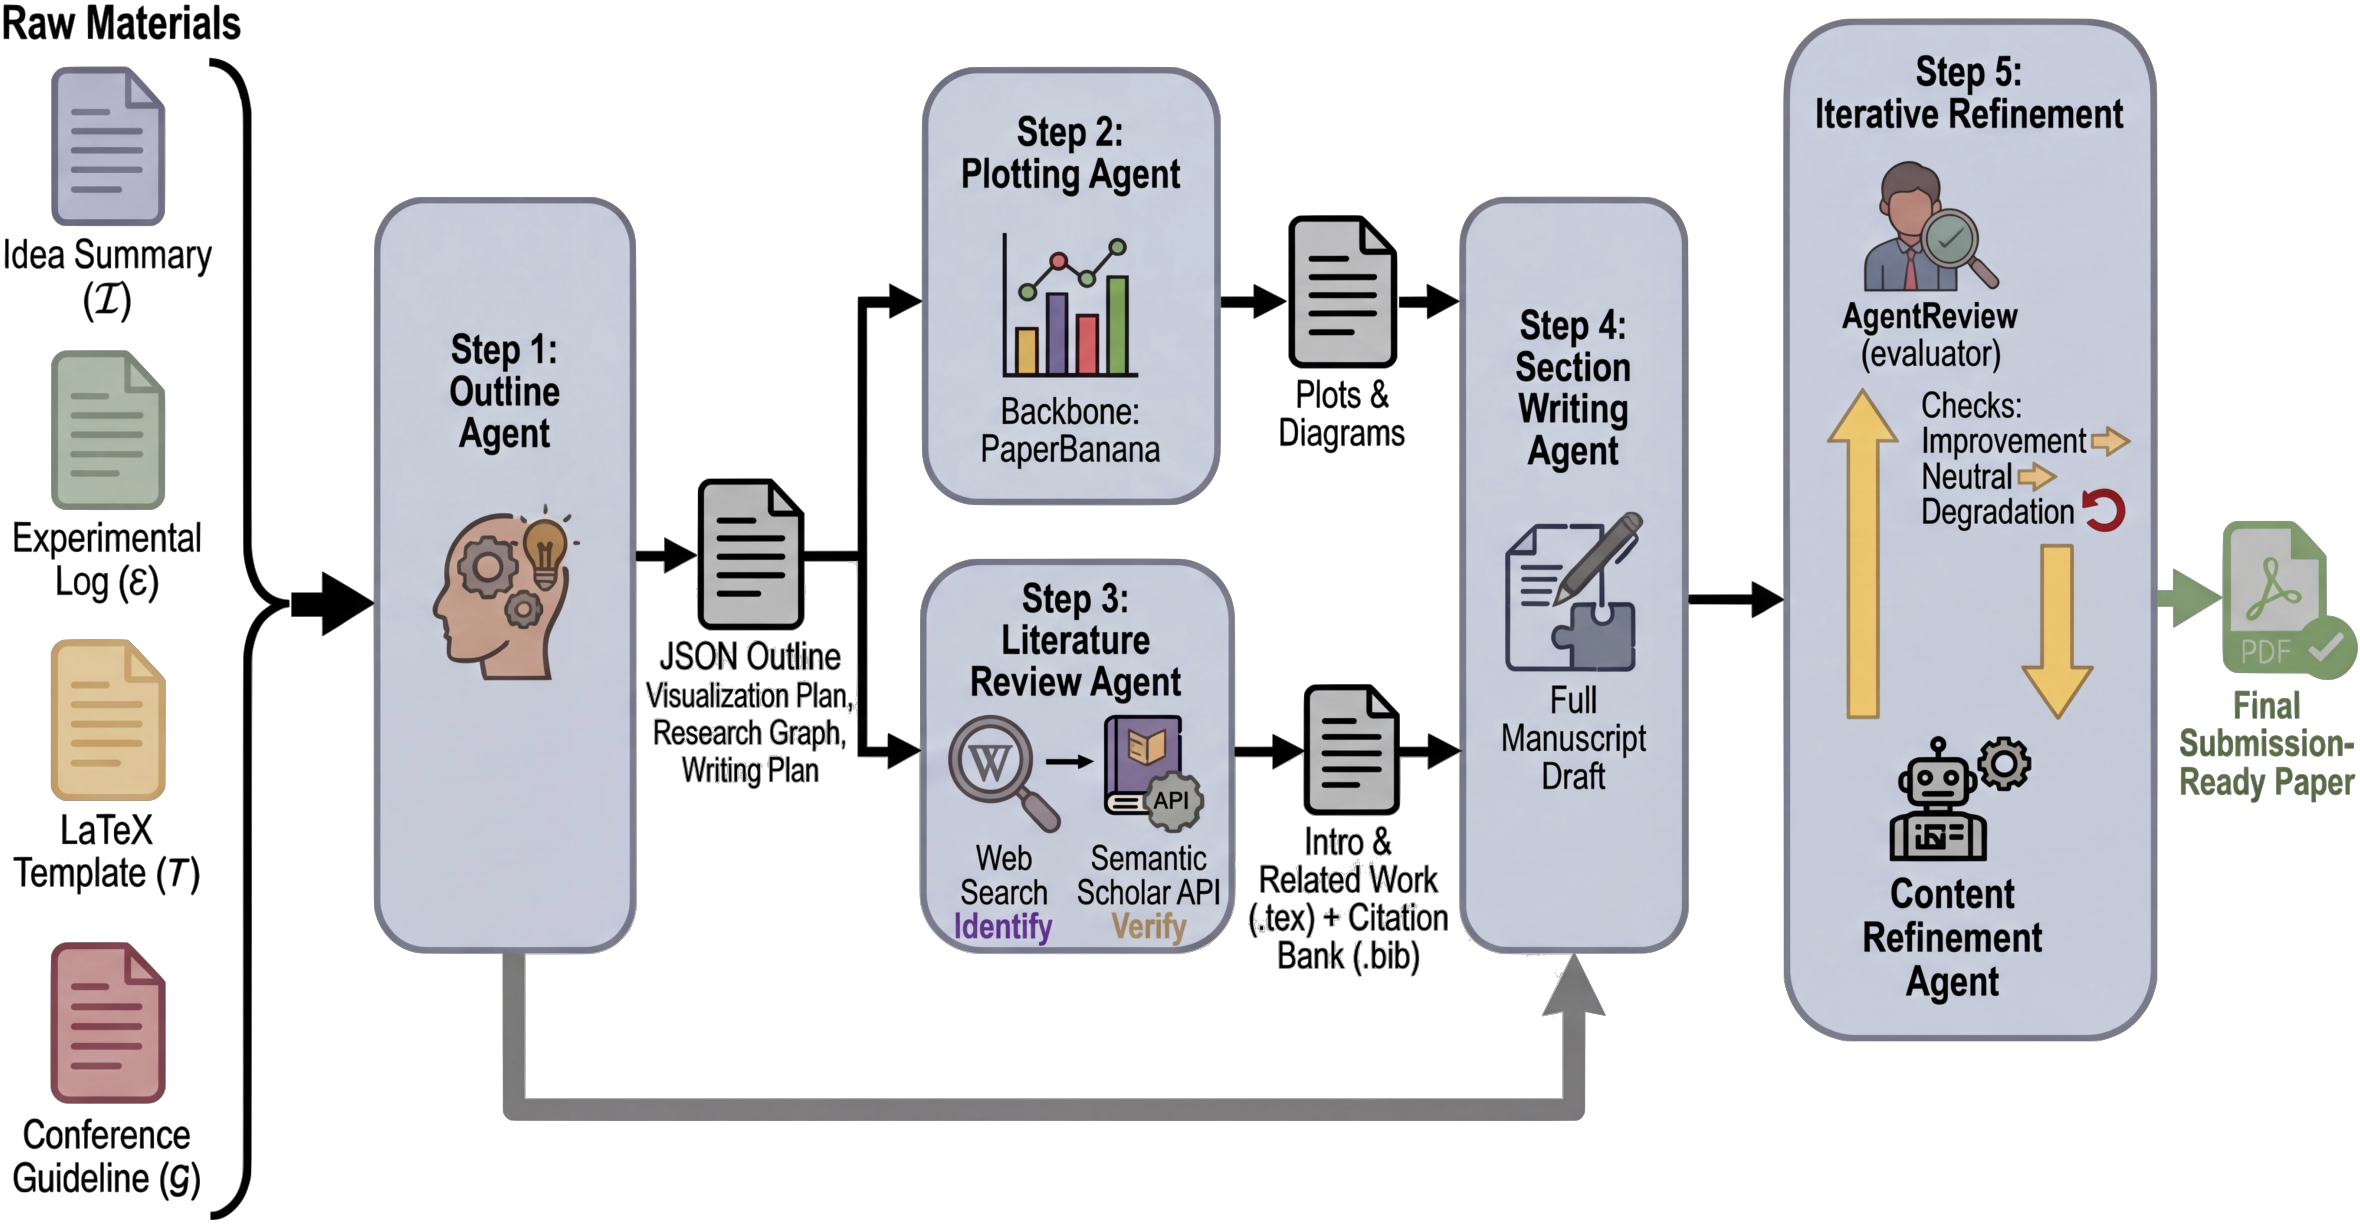
\includegraphics[width=0.95\linewidth]{content/figures/overview.png}
    \caption[Overview of the \ourmethod{} framework]{Overview of the \ourmethod{} framework. Specialized agents systematically parse unstructured inputs, synthesize plots and literature, compile a full draft, and iteratively refine the manuscript into a submission-ready PDF. (This figure was generated using PaperBanana~\citep{zhu2026paperbanana}.)}
    \label{fig:overview}
\end{figure}

Figure~\ref{fig:overview} illustrates \ourmethod, a multi-agent framework (App.~\ref{appendix:paper_writing_prompts}) that autonomously transforms pre-writing materials, including Idea Summary ($\mathcal{I}$), Experimental Log ($\mathcal{E}$), \mylatex{} Template ($\mathcal{T}$), and Conference Guidelines ($\mathcal{G}$), into submission-ready manuscripts. The pipeline executes five steps, with Step 2 and Step 3 operating in parallel:

\paragraph{Step 1: Outline Generation.} The \textit{Outline Agent} synthesizes pre-writing materials into a JSON outline comprising: (a) a visualization plan dictating specific plot types, data sources, and aspect ratios; (b) a targeted literature search strategy establishing both macro-level context and micro-level methodology clusters to guide the Literature Review Agent in conducting searches and constructing a citation map, which is subsequently leveraged to draft the \textit{Introduction} and \textit{Related Work} sections; and (c) a section-level writing plan including high-level content bullets and a comprehensive list of citation hints for all core external dependencies, such as baselines, datasets, and metrics used in the paper.

\paragraph{Step 2: Plot Generation.} The \textit{Plotting Agent} executes the visualization plan to generate conceptual diagrams and statistical plots. We use \textit{PaperBanana}~\citep{zhu2026paperbanana} as the default module, which employs a closed-loop refinement system where a VLM critic evaluates rendered images against design objectives, iteratively revising text descriptions and regenerating images to resolve visual artifacts, and synthesizing context-aware captions.

\paragraph{Step 3: Literature Review.} Executing the search strategy outlined in Step 1, the \textit{Literature Review Agent} drives a concurrent, hybrid discovery pipeline. It employs an LLM equipped with web search to identify candidate papers, then uses the Semantic Scholar API to authenticate their existence (App.~\ref{appendix:citation_verification}). Upon a successful match, the agent fetches the abstract and metadata while enforcing temporal cutoffs (App.~\ref{appendix:model_details}); candidates are discarded if they exceed the cutoff date or lack a verified mapping. Following deduplication via Semantic Scholar IDs, the agent compiles a citation registry and auto-generates a BibTeX (\texttt{.bib}) file. Finally, it uses the verified citations to draft the \textit{Introduction} and \textit{Related Work} sections.

\paragraph{Step 4: Section Writing.} The \textit{Section Writing Agent} drafts the remaining core sections using the outputs from previous stages. Building upon the partially filled \mylatex{} file, it extracts numeric values from the experimental log to construct tables. Guided by the section-level outline and the established citation bank, the agent authors the abstract, methodology, experiments, and conclusion sections, seamlessly integrating the generated figures to produce a complete \mylatex{} manuscript.

\paragraph{Step 5: Iterative Content Refinement.} The \textit{Content Refinement Agent} iteratively optimizes the manuscript using simulated peer-review feedback. Here we use \textit{AgentReview}~\citep{jin2024agentreview} as the default system in this module. After modifying the \mylatex{} source to address weaknesses, revisions are accepted if the overall score increases, or if it ties while net sub-axis gains are non-negative. The agent immediately reverts to the previous version and halts upon any overall score decrease, negative tie-breaker, or reaching the iteration limit. The resulting \mylatex{} document and compiled PDF represent the final output of \ourmethod.

